\documentclass[tikz,border=3pt]{standalone}
\usetikzlibrary{positioning,shapes.geometric,arrows.meta}
\begin{document}
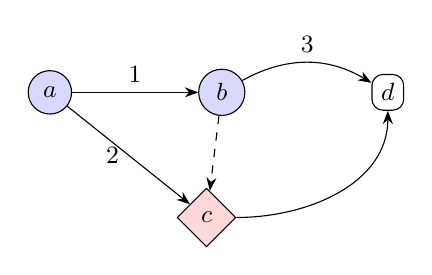
\begin{tikzpicture}[node distance=1.2cm and 1.6cm, every node/.style={font=\small}]
  \node[circle,draw,fill=blue!15] (a) {$a$};
  \node[circle,draw,fill=blue!15,right=of a] (b) {$b$};
  \node[diamond,draw,fill=red!15,below right=of a] (c) {$c$};
  \node[rectangle,draw,rounded corners,right=of b] (d) {$d$};
  \draw[-{Stealth}] (a) -- node[above] {1} (b);
  \draw[-{Stealth}] (a) -- node[left] {2} (c);
  \draw[-{Stealth},dashed] (b) -- (c);
  \draw[-{Stealth},bend left] (b) to node[above] {3} (d);
  \draw[-{Stealth}] (c) to[out=0,in=-90] (d);
\end{tikzpicture}
\end{document}
